
\section{Crear Maquina Virtual}

	\begin{center}
\item PASOS DE CREACIÓN  DE  UNA MAQUINA VIRTUAL EN VMWARE WORKSTATION 14 

    \end{center}
    
\end{itemize}


\begin{itemize}
\item PASO 1:
\\Una vez abierto el VMWare Workstation 14 hacemos clic en Crear una máquina virtual
		\begin{center}
		\includegraphics[width=15cm]{./Imagenes/1}
		\end{center}
	

	\end{itemize} 
	

	\begin{itemize}
\item PASO 2:
\\Seleccionamos la última opción avanzada y clic en Next.
		\begin{center}
		\includegraphics[width=15cm]{./Imagenes/2}
		\end{center}
	

	\end{itemize} 
	
	\begin{itemize}
\item PASO 3:
\\Hacemos clic en Next sin hacer ninguna configuración.
		\begin{center}
		\includegraphics[width=15cm]{./Imagenes/3}
		\end{center}
	

	\end{itemize} 
	
	\begin{itemize}
\item PASO 4:
\\Seleccionamos la última opción  porque aún no tenemos el instalador y clic en Next
		\begin{center}
		\includegraphics[width=15cm]{./Imagenes/4}
		\end{center}
		\\\
	\end{itemize} 
	
	
	\begin{itemize}

\item PASO 5:
\\Seleccionamos  el tipo de sistema operativo Linux y la versión CentOS 6 y clic en Next.
		\begin{center}
		\includegraphics[width=15cm]{./Imagenes/5}
		\end{center}
	

	\end{itemize} 

	\begin{itemize}
\item PASO 6:
\\Escribimos un nombre y fijamos la dirección de la máquina virtual y clic en Next.
		\begin{center}
		\includegraphics[width=15cm]{./Imagenes/6}
		\end{center}
		\\\

	\end{itemize} 

	\begin{itemize}
\item PASO 7:
\\Colocamos 1 GB de memoria RAM como mínimo y clic en Next.
		\begin{center}
		\includegraphics[width=15cm]{./Imagenes/7}
		\end{center}
	

	\end{itemize} 

	\begin{itemize}
\item PASO 8:
\\Seleccionamos la tarjeta de red en este caso bridged networking y clic en Next.
		\begin{center}
		\includegraphics[width=15cm]{./Imagenes/8}
		\end{center}
	

	\end{itemize} 

	\begin{itemize}
\item PASO 9:
\\Lo dejamos seleccionado en LSI Logic (Recommended) y clic en Next.
		\begin{center}
		\includegraphics[width=15cm]{./Imagenes/9}
		\end{center}
	

	\end{itemize} 

	\begin{itemize}
\item PASO 10:
\\Seleccionamos SCSI (Recommended) y clic en Next.
		\begin{center}
		\includegraphics[width=15cm]{./Imagenes/10}
		\end{center}
	

	\end{itemize} 

	\begin{itemize}
\item PASO 11:
\\Seleccionar la primera opción donde crearemos una nueva máquina virtual y clic en Next.\\
		\begin{center}
		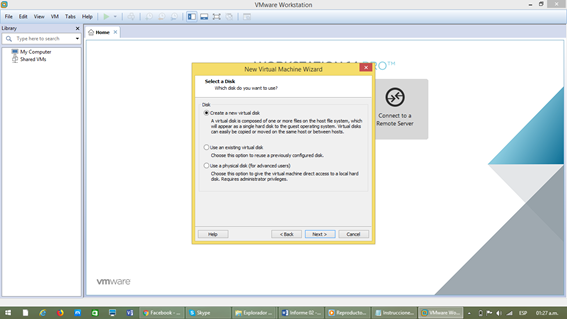
\includegraphics[width=15cm]{./Imagenes/11}
		\end{center}
	

	\end{itemize} 

	\begin{itemize}
\item PASO 12:
\\Definimos el tamaño de disco en este caso es 60 GB y clic en Next.\\
		\begin{center}
		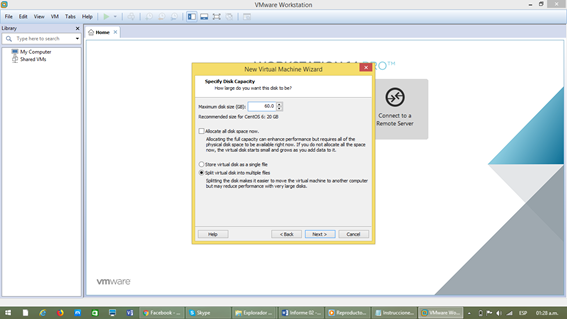
\includegraphics[width=15cm]{./Imagenes/12}
		\end{center}
	

	\end{itemize} 

	\begin{itemize}
\item PASO 13:
\\Una vez terminado nos va a mostrar un resumen de las características de la nueva máquina virtual CentOS 6.2 y clic en Finish.
\\
		\begin{center}
		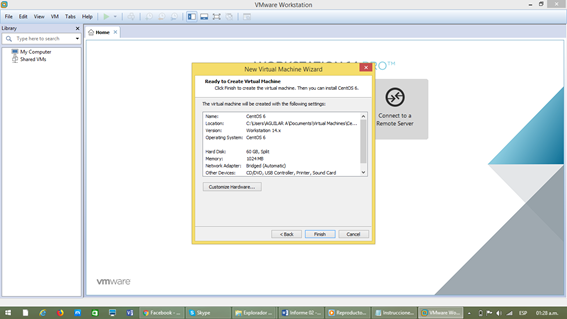
\includegraphics[width=15cm]{./Imagenes/13}
		\end{center}
	

	\end{itemize} 

	\begin{itemize}
\item PASO 14:
\\Finalmente tenemos nuestra máquina virtual creada y sus características.\\
		\begin{center}
		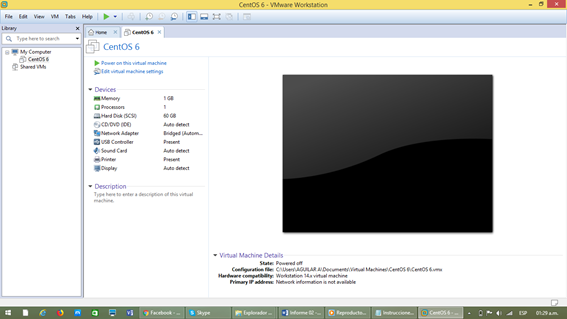
\includegraphics[width=15cm]{./Imagenes/14}
		\end{center}
	

	\end{itemize} 



\begin{itemize}


  \end{itemize}
  
  

